\chapter{Prototype}
The prototype consist of an RMI distributed application, which contains the necessary functionality; registering remote objects in a registry in which clients are able to invoke these registered objects remotely.

To further enhance the capability of anRMI distributed application, the prototype is implemented with 2 different algorithms, Bully Election Algorithm and Ring Election Algorithm.

Such leader elections, allows for an ongoing distribution of data even when a client/server terminates within in a DDS is terminated, allowing fault tolerance.

This chapter describes the process of implementing the prototype, and at the end, evaluating the algorithms within the RMI application.

\subsection{Analysis}
During the analysis phase, we took in notes about the fundamentals of RMI applications and devised a simple strategy of implmenting the distributed application, by taking the guide into consideration, given by Oracle's introduction to RMI, and the given requirements for the application.

\begin{figure}[ht!]
\centering
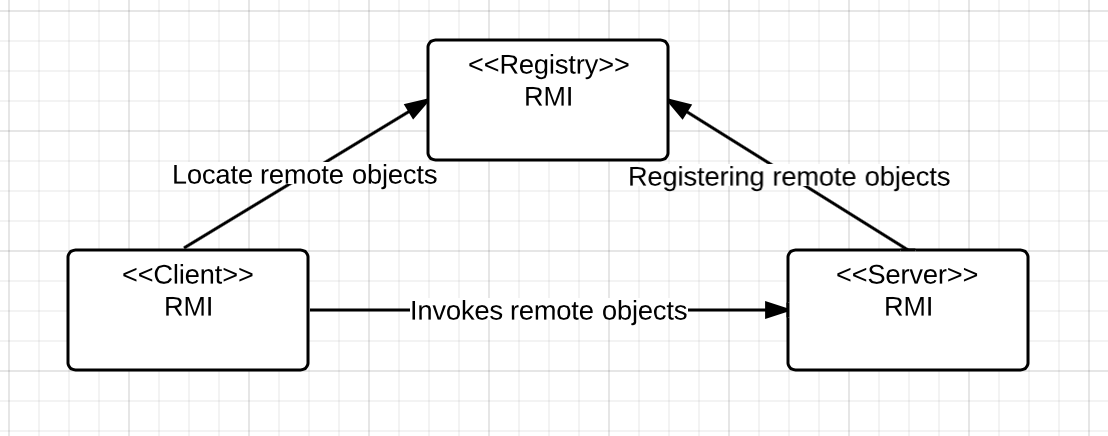
\includegraphics[width=80mm]{img/analyze_diagram.png}
\caption{Analyzing phase - diagram overview.}
\label{Analyzing phase}
\end{figure}

\subsection{Implementation}
For the implementation of the RMI application, it consist of 3 java classes, as seen on Figure 3.2. The NodeRemoteInterface.java extends the Remote to allow allocation of remote methods for implementation of the remote objects, namely, Node.java. 

Node.java contains methods that allows for registering of the node, and specify the election procedure. Further more the nodes required to extends its capabilities by extending the election procedure to follow a certain algorithm, namely Bully Algorithm and Ring Algorithm.

The Program.java is the program itself to execute and register the node to RMI registry and for the purpose of testing the RMI application by explicit sending messages and test the different Leader Election; Bully Algorithm and Ring Algorithm.

\begin{figure}[ht!]
\centering
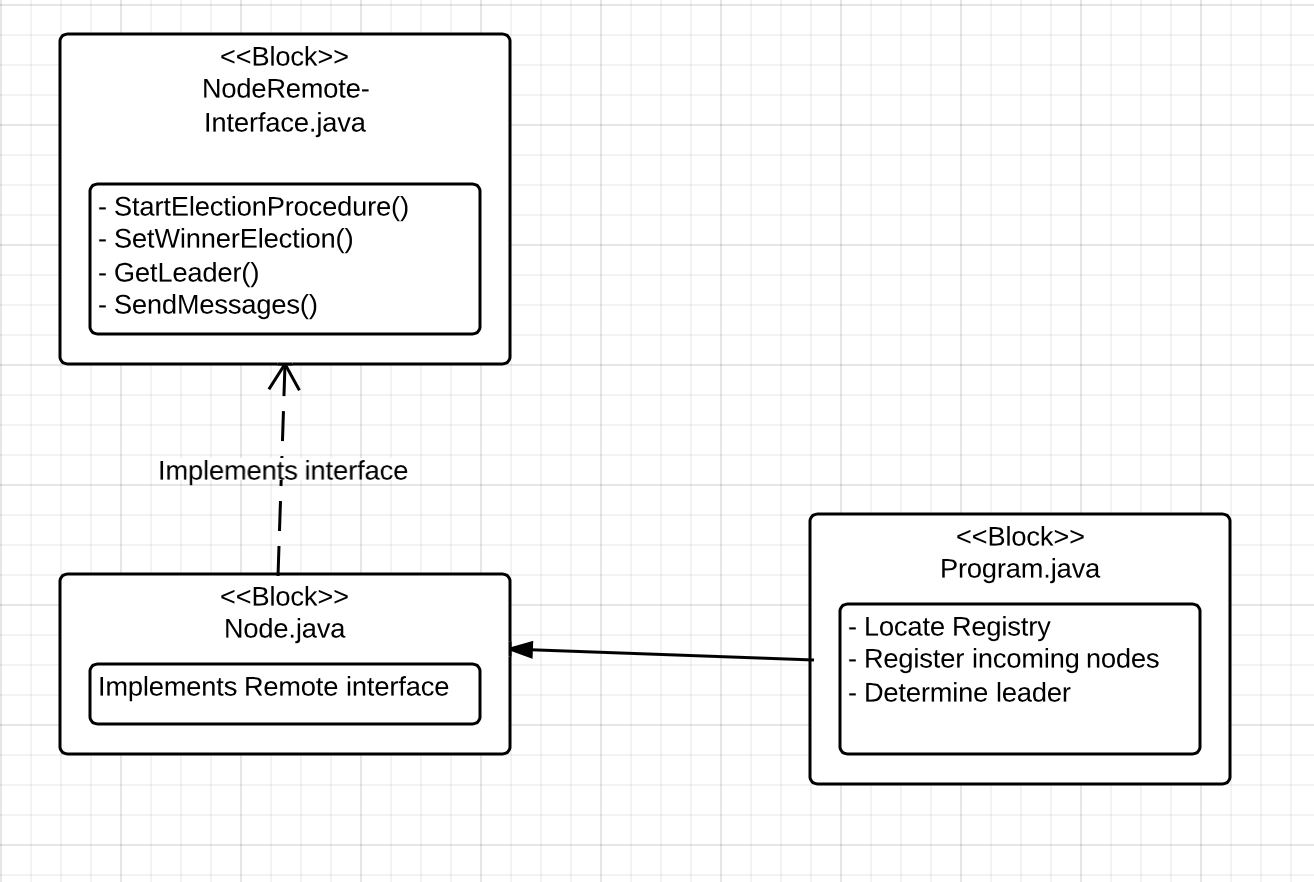
\includegraphics[width=80mm]{img/Implementation_uml_diagram.png}
\caption{Implementation of RMI - UML diagram.}
\label{Implementation of RMI - UML diagram}
\end{figure}

\subsubsection{Implementation of Bully Algorithm}
Codesnippet of Bully Algorithm.

\begin{figure}[ht!]
\centering
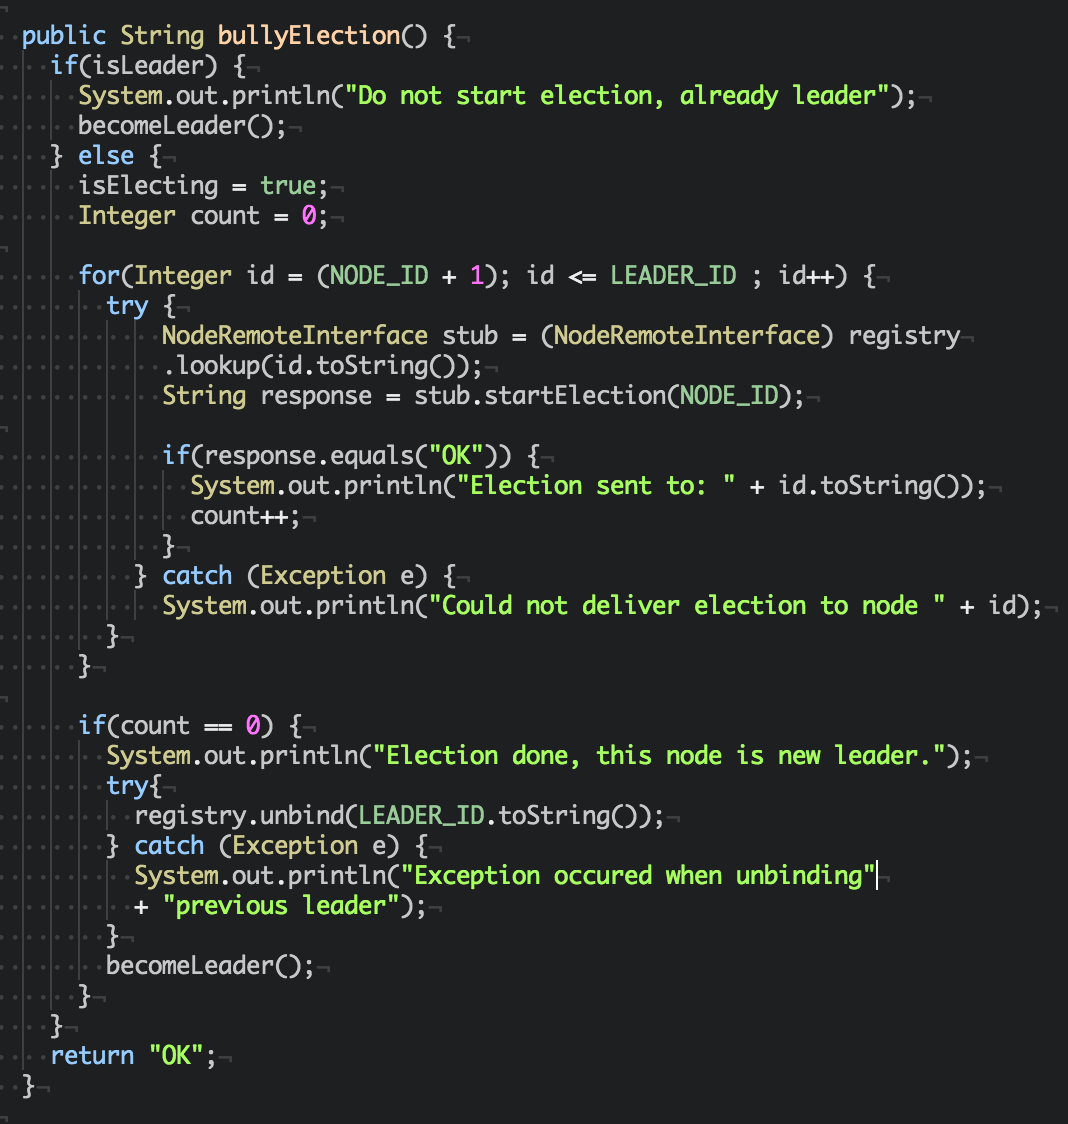
\includegraphics[width=80mm]{img/bully_election_code.png}
\caption{Codesnippet of Bully Algorithm}
\label{Codesnippet of Bully Algorithm}
\end{figure}

\newpage

\subsubsection{Implementation of Ring Algorithm}
Codesnippet of Ring Algorithm.

\begin{figure}[ht]
\centering
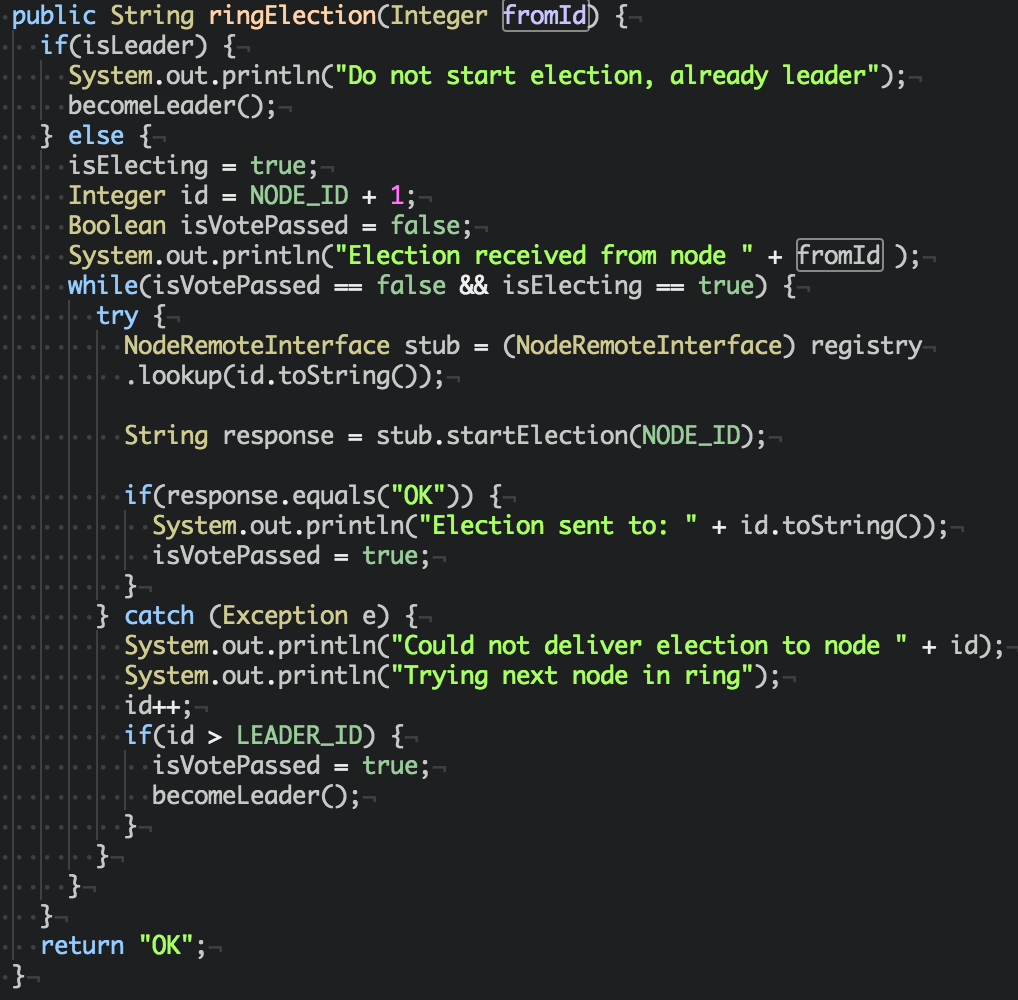
\includegraphics[width=80mm]{img/ring_election_code.png}
\caption{Codesnippet of Ring Algorithm}
\label{Codesnippet of Ring Algorithm}
\end{figure}


\subsection{Test}

The Figure, shows the execution of starting different nodes and handing out node ID for each incoming nodes that joins the RMI application. Further more for each addition of nodes, it handles the election procedure and always give the highest ID node the leader role.

\begin{figure}[ht!]
\centering
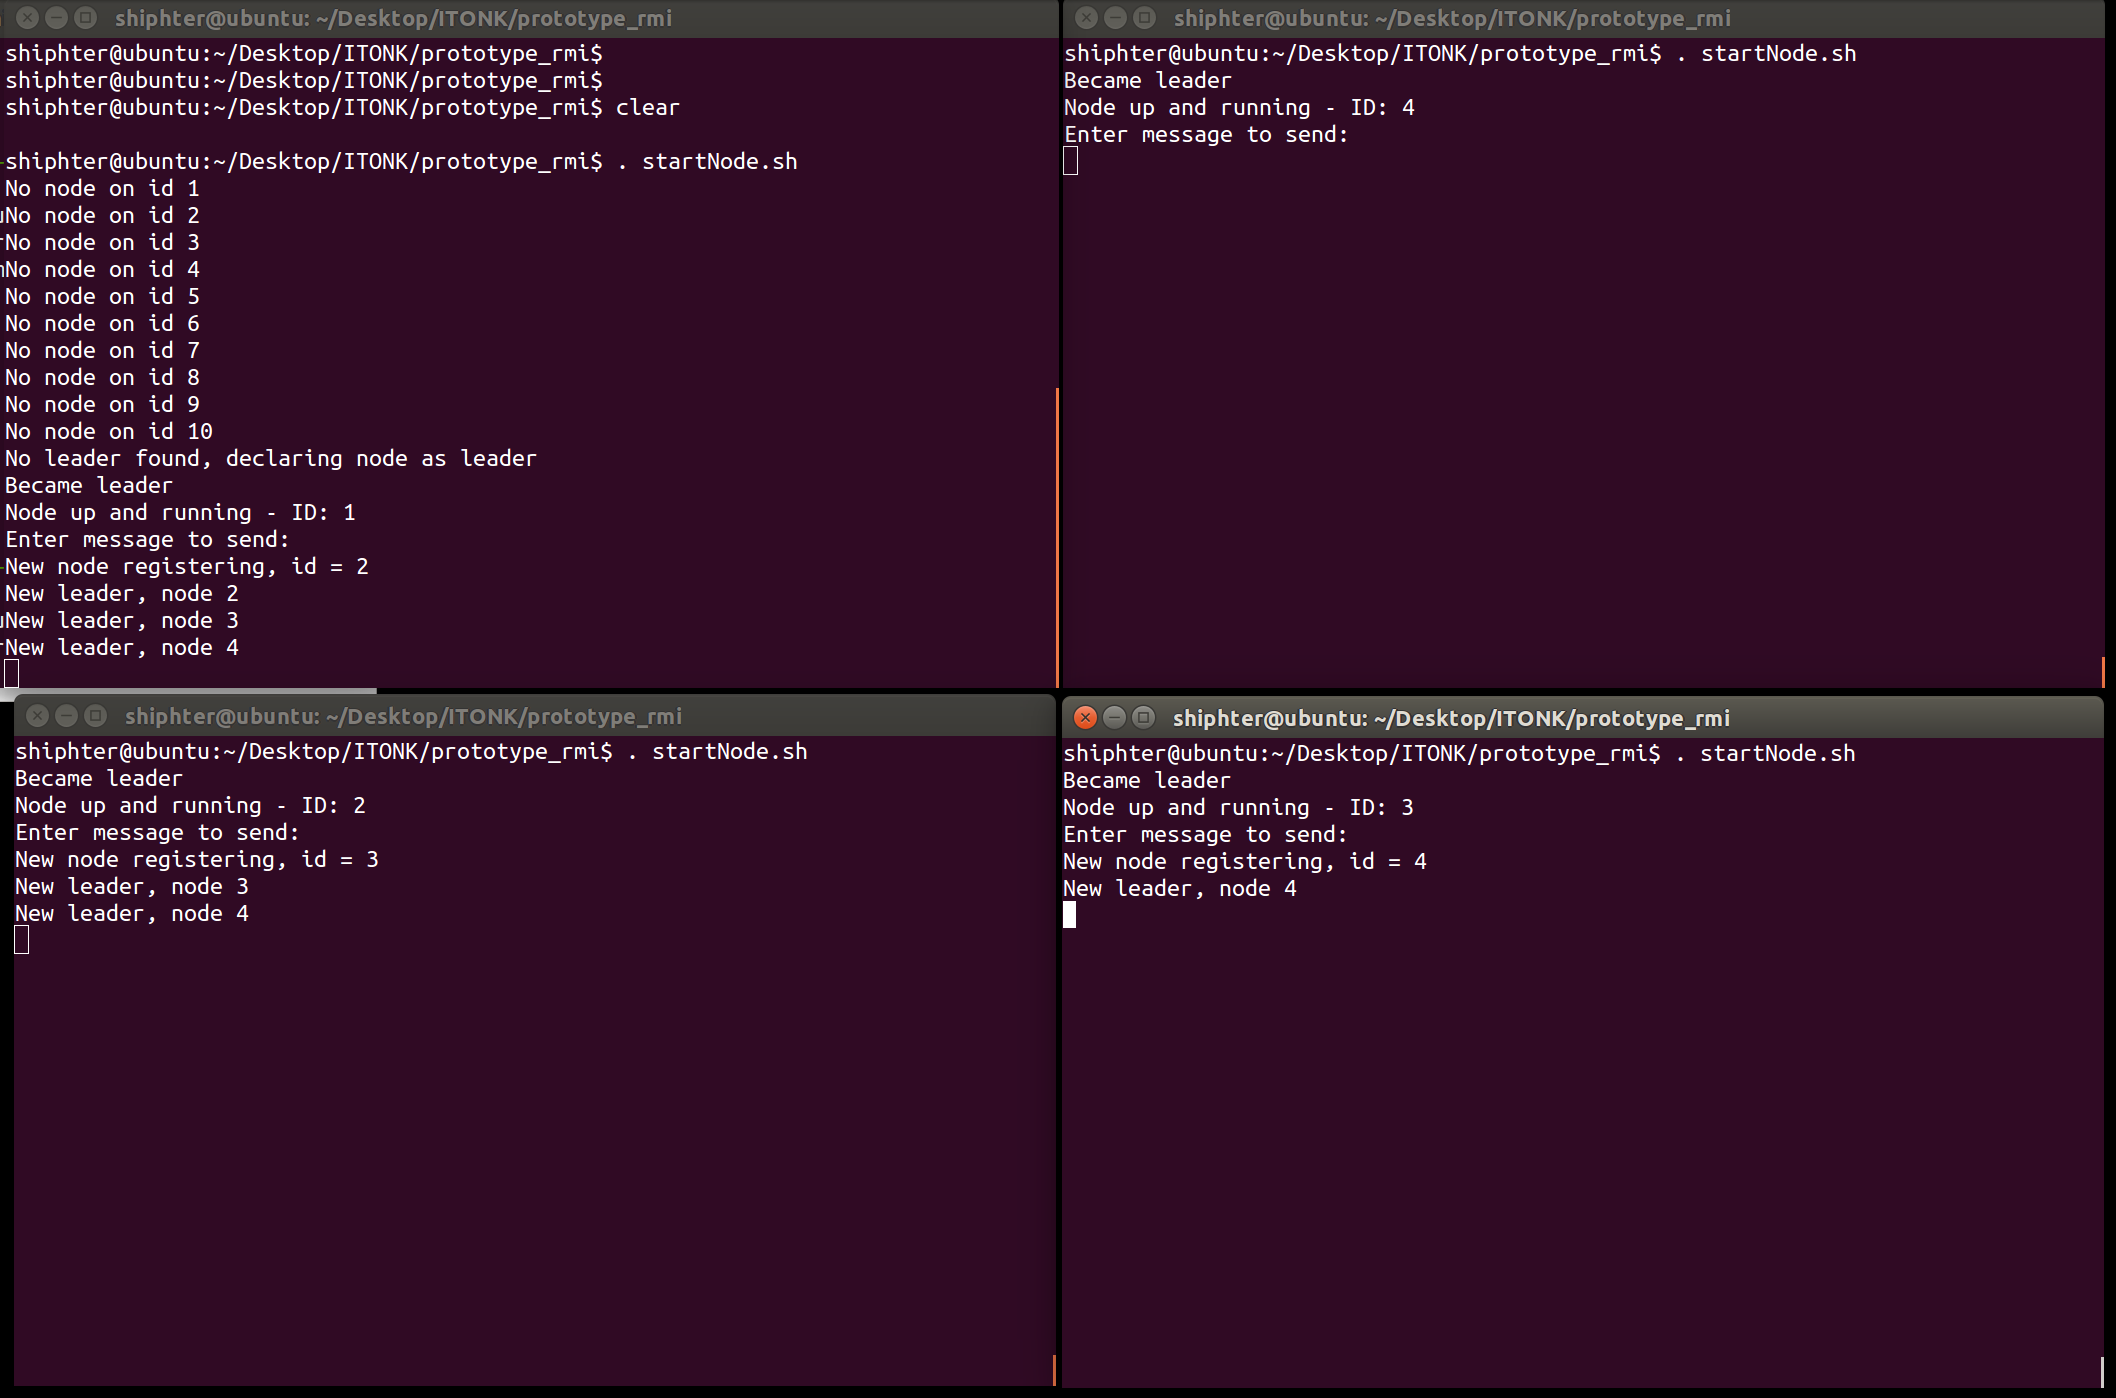
\includegraphics[width=80mm]{img/starting_nodes.png}
\caption{Test of starting nodes}
\label{Test of starting Nodes}
\end{figure}

\newpage

The next Figure shows the improved version of leader election, namely, Bully Election, and is working as intended, as when the leader stops responding, the election procedure begins and finishes by aquiring the leader to the highest ID number node.

\begin{figure}[ht!]
\centering
\caption{Test of Bully Election}
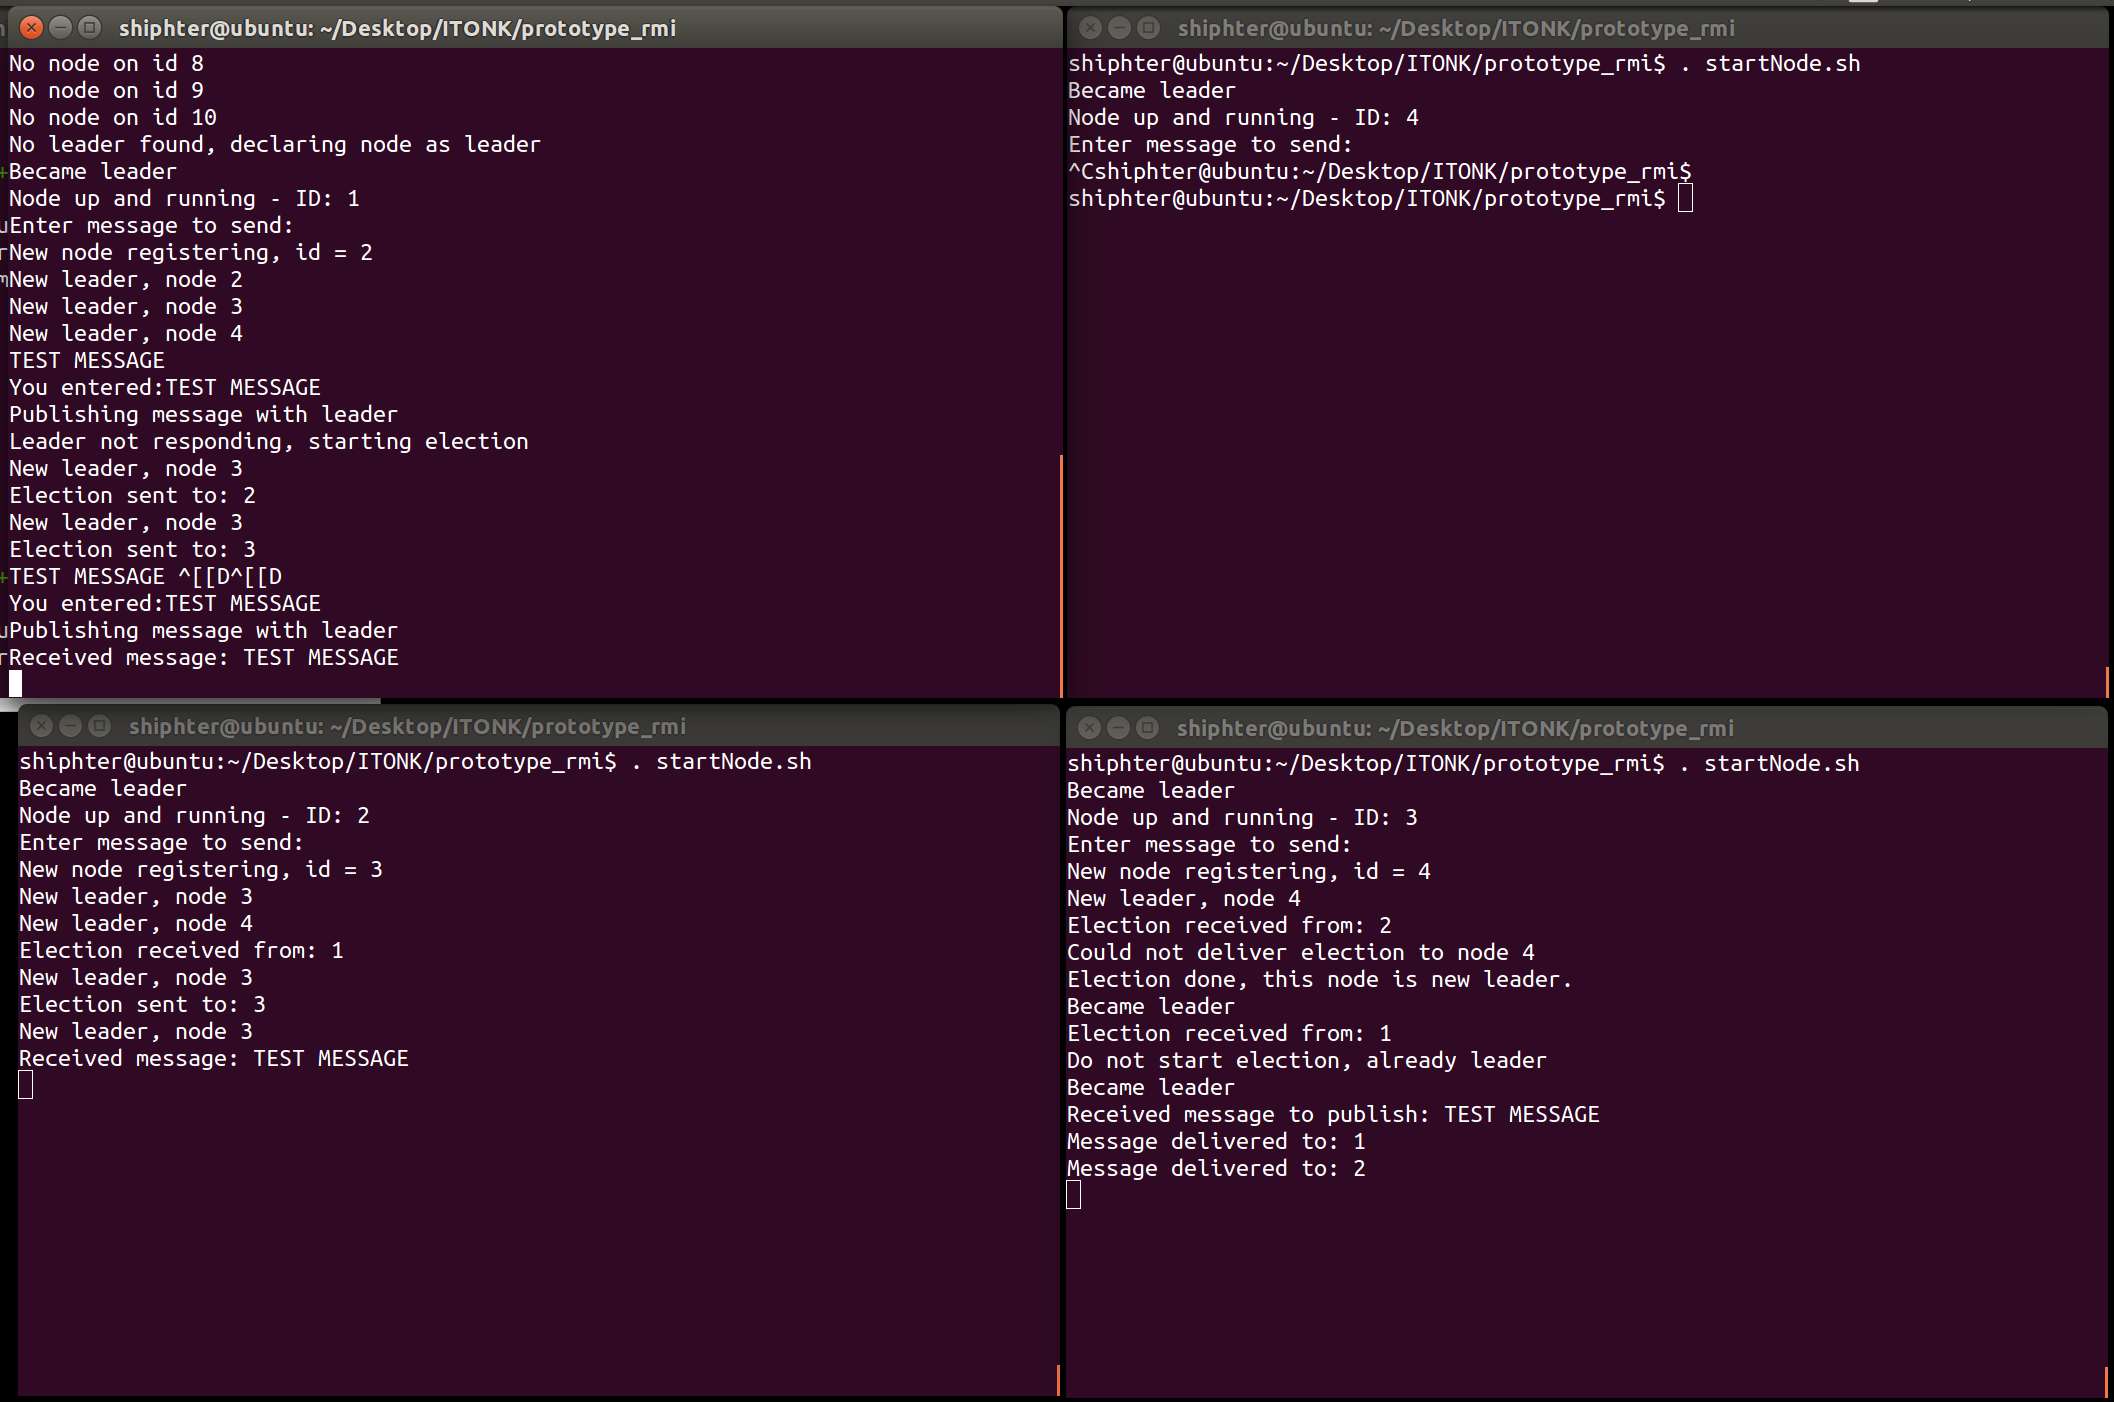
\includegraphics[width=80mm]{img/bully_election_messages.png}
\label{Test of Bully Election}
\end{figure}

The next Figure shows the Ring election, with the procedure of giving an election for a nodes next successor in regard to its ID number. As seen on the message, a node is skipped because of a broken node and the next node is notified with the election, and each node has then been giving an updated list of nodes that is online.

\begin{figure}[ht!]
\centering
\caption{Test of starting nodes}
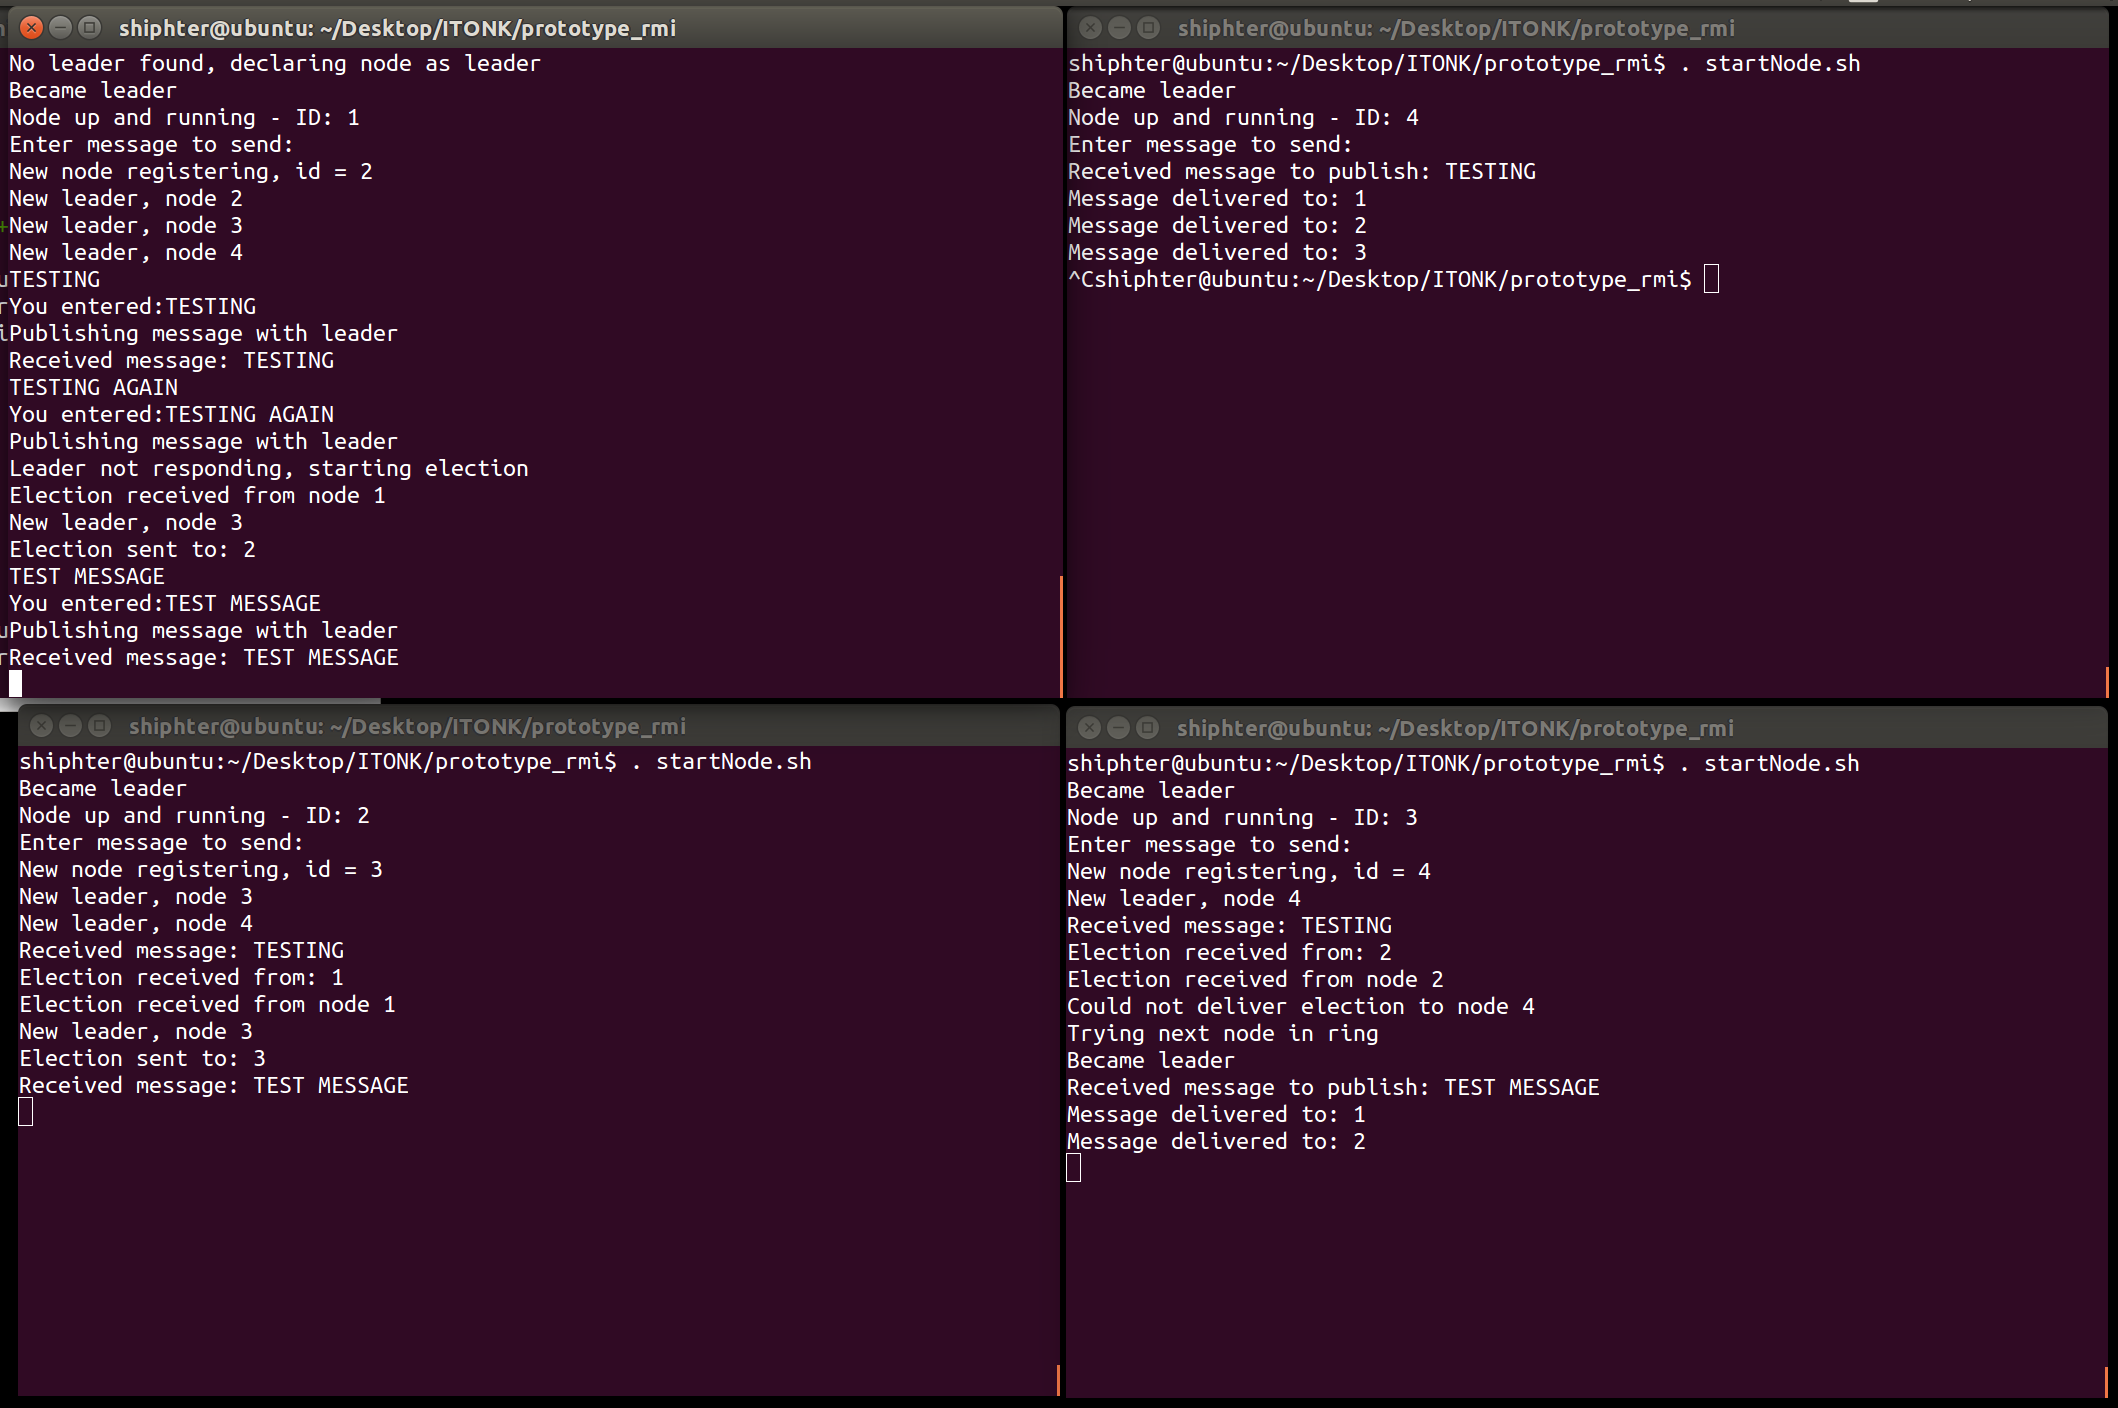
\includegraphics[width=80mm]{img/ring_election_messages.png}
\label{Test of Ring Election}
\end{figure}











